\documentclass{standalone}
\usepackage{tikz}
\usetikzlibrary{angles,quotes,math}

\begin{document}
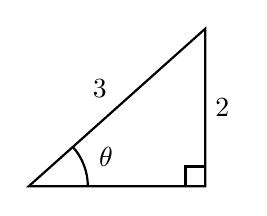
\begin{tikzpicture}[thick]
  \coordinate (a) at (0,0);
  \coordinate (b) at (2.24,2);
  \coordinate (c) at (2.24,0);
  \draw
  (a) pic["\(\theta\)", draw=black, -, angle eccentricity=1.4, angle radius=0.75cm]
  {angle=c--a--b} -- node[above left] {\(3\)}
  (b) -- node[right] {\(2\)}
  (c) -- cycle;
  % Right angle square
  \draw (c) rectangle ++(-0.25,0.25);
\end{tikzpicture}
\end{document}
